\paragraph*{Устойчивость системы\\}
\hspace*{\parindent}Система называется устойчивой, если после снятия внешнего возмущения она возвращается в исходное состояние. Так как движение системы в свободном состоянии описывается однородным дифференциальным уравнением, то математическое определение устойчивой системы можно сформулировать следующим образом: 
\begin{equation}\label{needed}
	\lim_{t \to \infty} y_{o}(t) = 0,
\end{equation}
где $y_{o} = \sum_{k=1}^{n} C_ke^{\lambda_kt}$ - общее решение дифференциального уравнения, $\lambda = \sigma+i\omega$ - корень характеристического полинома.

Соответственно, для выполнения условия \eqref{needed} необходимо, чтобы вещественная часть $\sigma$ всех корней $\lambda$ характеристического полинома дифференциального уравнения была меньше нуля. 

Так как знаменатель передаточной функции является характеристическим полиномом, а его корни - полюсами, то критерием устойчивости для системы, заданной передаточной функцией, является нахождение \textit{всех} его полюсов в левой полуплоскости  комплексной плоскости $s$. Именно в этом заключается критерий устойчивости Найквиста-Михайлова.

Очевидно, что для достижения желаемого результата замкнутые системы регуляторов \eqref{pidfunc} и \eqref{pifunc} должны быть устойчивыми. Для этого коэффициенты регуляторов должны быть такими, чтобы корни характеристических полиномов лежали в левой полуплоскости $s$. Распространенным способом достижения этого требования является приравнивание характеристического полинома к полиному с известными корнями.

\paragraph*{Бином Ньютона\\}
\hspace*{\parindent}Одним из таких полиномов является бином Ньютона, имеющий следующий вид: 
\begin{equation}\label{newt}
	D^*(\lambda)=(\lambda+\omega_0)^n,
\end{equation}
где $\omega_0 > 0$.

Как видно из выражения \eqref{newt}, бином имеет отрицательные вещественные кратные корни, которые равны:
\begin{equation}
	\lambda_i=-\omega_0, \phantom{-}i=\overline{1,n},
\end{equation}

\begin{figure}[h]
	\noindent\centering{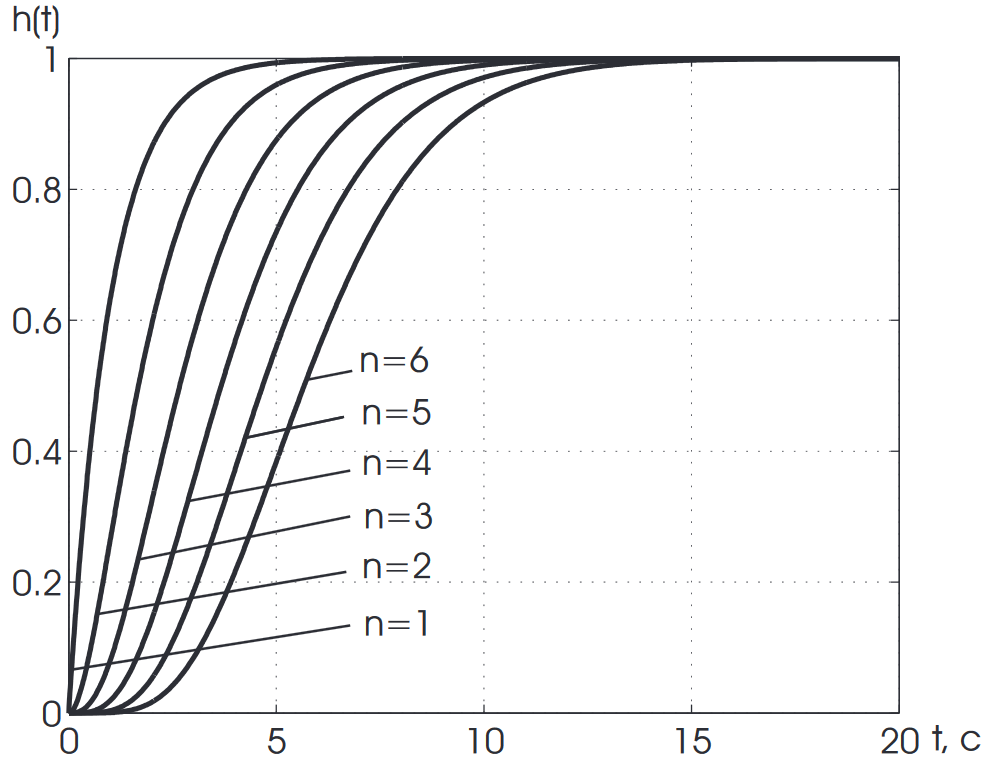
\includegraphics[height = 6cm]{img/newph.png}}
	\caption{Нормированные переходные характеристики полинома Ньютона}
	\label{newgraph}
\end{figure}

Такие корни характеристического полинома в теории обеспечивают апериодический характер переходных процессов, то есть с нулевым перерегулированием, однако в реальных системах управления достижение нулевого значения перерегулирования является весьма сложной задачей. Во многих случаях в системе присутствует перерегулирование, которое обусловлено инерционностью объекта управления.\\

Биномы Ньютоны с первого по третий порядок системы представлены в таблице:
\begin{center}
\begin{tabular}{ |c|c| } 
 \hline
 Порядок системы &  Стандартный полином Ньютона \\ 
 \hline
 1 & $\lambda+\omega_0$ \\ 
 \hline
 2 & $\lambda^2+2\omega_0\lambda+\omega_0^2$ \\ 
 \hline
 3 & $\lambda^3+3\omega_0\lambda^2+3\omega_0^2\lambda+\omega_0^3$ \\ 
 \hline
\end{tabular}\\
\end{center}

Соответственно, для системы \eqref{pidfunc} с характеристическим полиномом 3-го порядка можно записать:
\begin{equation}
	J_ms^3+(K+k_d)s^2+k_ps+k_i = s^3+\frac{(K+k_d)s^2}{J_m}+\frac{k_ps}{J_m} +\frac{k_i}{J_m} =(s+\omega_0)^3= s^3+3\omega_0s^2+3\omega_0^2s+\omega_0^3,
\end{equation}
откуда можно получить желаемые значения коэффициентов регулятора:
\begin{equation}
	k_p = 3\omega_0^2J_m, \phantom{- }k_i = \omega_0^3J_m, \phantom{- } k_d=3\omega_0J_m - K
\end{equation}

Аналогично для системы \eqref{pifunc}:
\begin{equation}
	J_ms^2+(K+k_p^1)s+k_i^1 = s^2+\frac{(K+k_p^1)s}{J_m}+\frac{k_i^1}{J_m} =(s+\omega_0)^2= s^2+2\omega_0s+\omega_0^2,
\end{equation}
откуда:
\begin{equation}
	k_p^1 = 2\omega_0J_m-k, \phantom{- }k_i^1 = \omega_0^2J_m
\end{equation}

Для формирования полинома Ньютона необходимо знать значение параметра $\omega_0$.  Определить этот параметр позволяет метод стандартных переходных функций основанный на нормированных переходных функциях. Нормированные переходные функции имеет только полюса, получаются путем замены значения параметра $\omega_0$ на единицу в формулах, определяющих полином Ньютона, и имеют вид:
%Проверь мысли свои как формулируешь
\begin{equation}
	W(s) = \frac{1}{D^*(s)}, \phantom{-} \omega_0=1
\end{equation}

Графики нормированных переходных функций, получаемые при подаче единичного воздействия на вход системы, для случая бинома Ньютона представлены на рис.~\ref{newgraph}

\begin{figure}[h]
	\noindent\centering{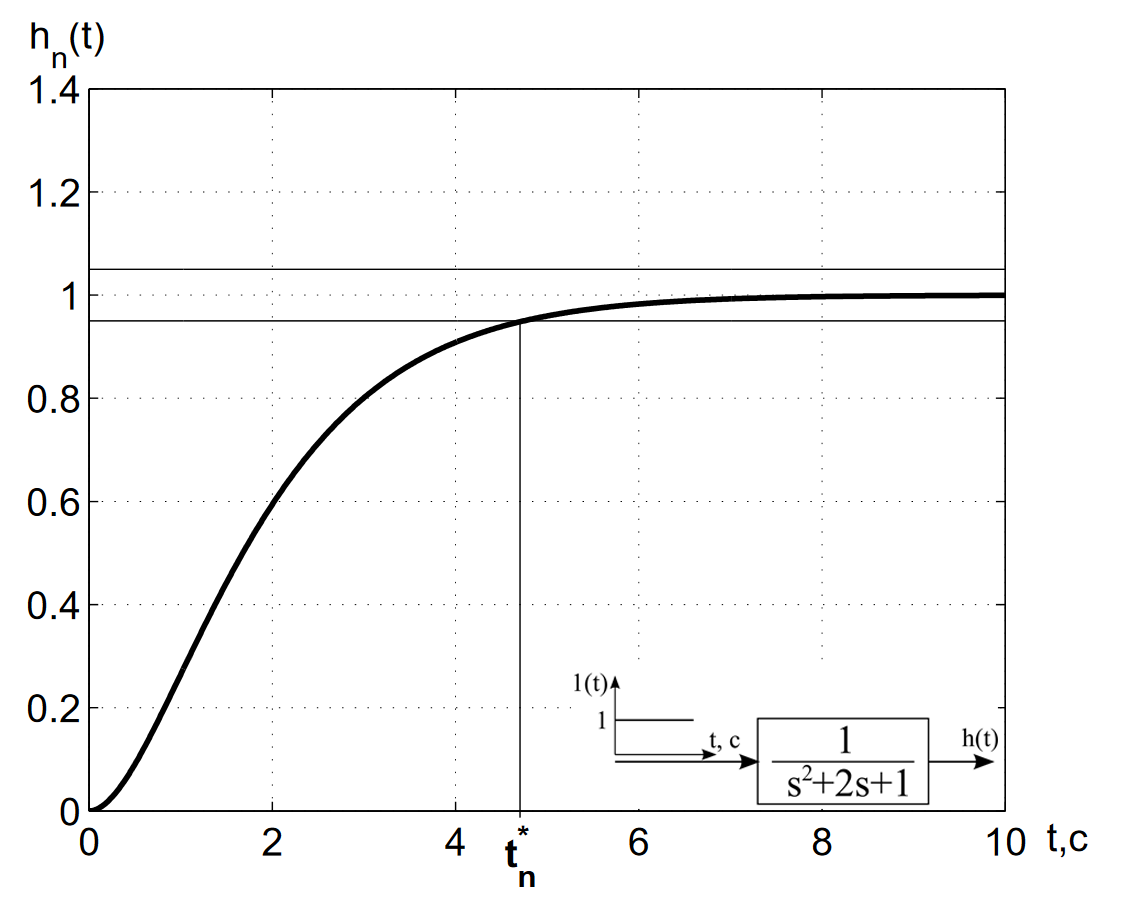
\includegraphics[height = 6cm]{img/newtime.png}}
	\caption{Определение времени переходного процесса }
	\label{newtime}
\end{figure}

Для нахождения требуемого характеристического полинома нужно определить время переходного процесса $t_n^*$, то есть определение момента времени, когда переходный процесс попадает в $\Delta$-область и больше её не покидает, где $\Delta$-область находится в приделах от 0,01\% до 0,05\% от установившегося значения переходного процесса. Нахождение  $t_n^*$ изображено на рис.~\ref{newtime}.

В таблице приведены $t_n^*$ для биномов Ньютона с 1-й по 3-й порядок:
\begin{center}
\begin{tabular}{ |c|c|c|c| } 
 \hline
 n &  1 & 2 & 3  \\ 
 \hline
 $t_n^*, c$ &  3.0 & 4.8 & 6.3  \\ 
 \hline
 $\sigma, \%$ &  0 & 0 & 0  \\ 
 \hline
\end{tabular}
\end{center}
где $\sigma$ - процент перерегулирования. 

Зная $t_n^*$ , на основе данного в техническом задании времени переходного процесса $t_n$, $\omega_0$ находится по формуле: 
\begin{equation}\label{omeganul}
	\omega_0=\frac{t_n^*}{t_n},
\end{equation}
основанной на принципе подобия, состоящего в том, что увеличение параметра $\omega_0$ приводит к увеличению скорости протекания процессов в системе, но при этом не оказывает влияния на колебательность этих процессов.

Результаты моделирования систем \eqref{pidfunc} и \eqref{pifunc} с коэффициентами, полученными из бинома Ньютона изображены на рис.~\ref{pidmod} и рис.~\ref{pimod} соответственно.

\begin{figure}[h]
	\noindent\centering{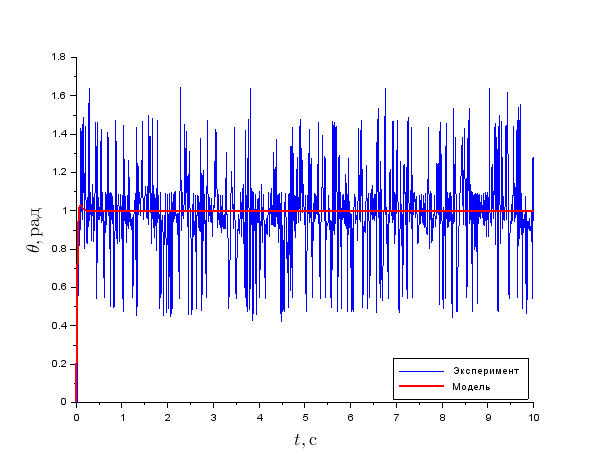
\includegraphics[height = 6cm]{img/N1.png}}
	\caption{График ПИД-регулятора с коэффициентами, полученными из бинома Ньютона при времени переходного процесса 0.1 сек }
	\label{pidmod}
\end{figure}

\begin{figure}[h]
	\noindent\centering{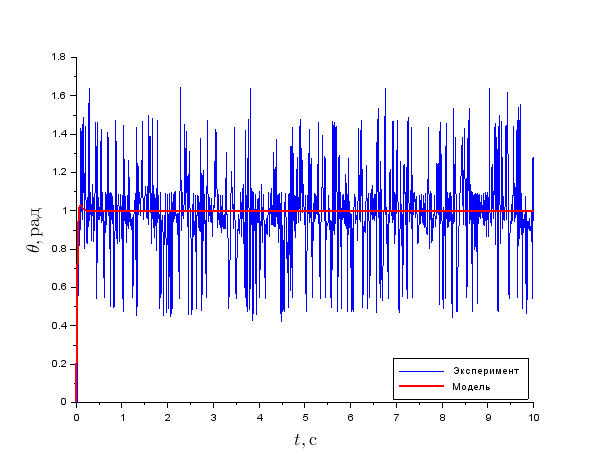
\includegraphics[height = 6cm]{img/N1.png}}
	\caption{График ПИ-регулятора с коэффициентами, полученными из бинома Ньютона при времени переходного процесса 0.1 сек }
	\label{pimod}
\end{figure}

\paragraph*{Полином Баттерворта\\}
\hspace*{\parindent}Еще одним полиномом, применяемым для нахождения коэффициентов, является полином Баттерворта, выражаемый следующим образом: 
\begin{equation}
	D^*(\lambda)=\prod_{i=1}^{n}(\lambda-\lambda_i^*).
\end{equation}
Его корни расположены в левой полуплоскости $s$ на полуокружности с радиусом $\omega_0$ и находятся по формуле:
\begin{equation}
	\lambda_i^*=\omega_0(\cos{\frac{\pi(2i-1)}{n}}+j\sin{\frac{\pi(2i-1)}{n}}),\phantom{-}i=\overline{1,n}.
\end{equation}\begin{figure}[h]
	\noindent\centering{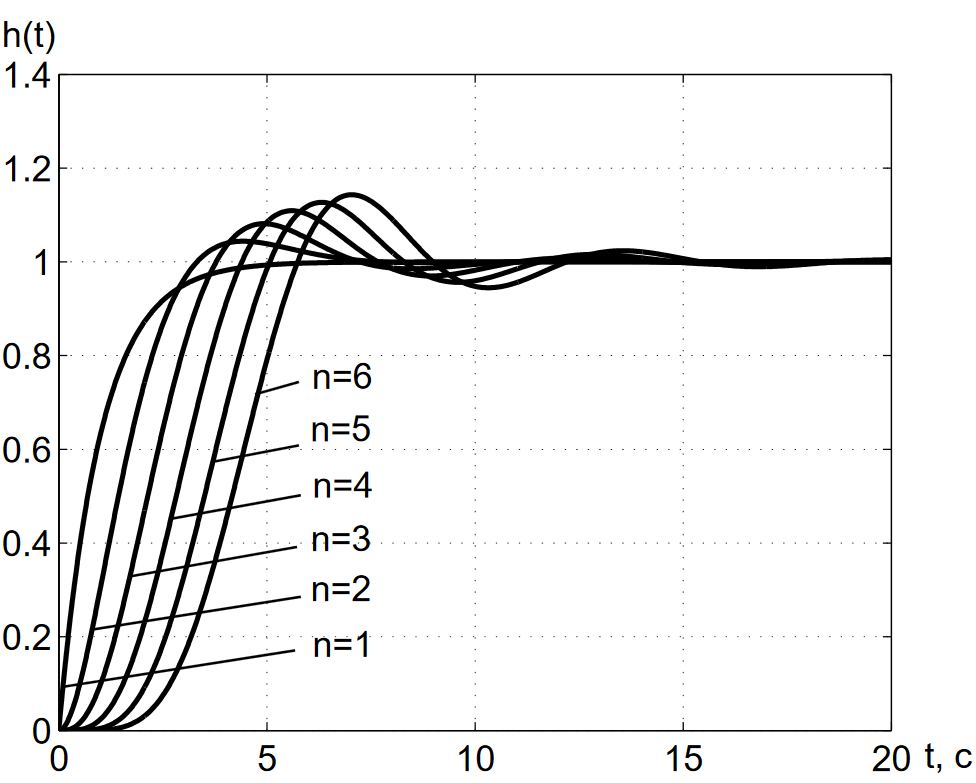
\includegraphics[height = 6cm]{img/buttergraph.png}}
	\caption{Нормированные переходные характеристики полинома Баттерворта}
	\label{buttergraph}
\end{figure}

Полиномы Баттерворта с первого по третий порядок системы представлены в таблице:
\begin{center}
\begin{tabular}{ |c|c| } 
 \hline
 Порядок системы &  Стандартный полином Баттерворта \\ 
 \hline
 1 & $\lambda+\omega_0$ \\ 
 \hline
 2 & $\lambda^2+1.4\omega_0\lambda+\omega_0^2$ \\ 
 \hline
 3 & $\lambda^3+2\omega_0\lambda^2+2\omega_0^2\lambda+\omega_0^3$ \\ 
 \hline
\end{tabular}
\end{center}

Коэффициенты системы находятся по такому же принципу, как и в случае с биномом Ньютона:
\begin{equation}
	J_ms^3+(K+k_d)s^2+k_ps+k_i = s^3+\frac{(K+k_d)s^2}{J_m}+\frac{k_ps}{J_m} +\frac{k_i}{J_m} =(s+\omega_0)^3= s^3+2\omega_0s^2+2\omega_0^2s+\omega_0^3,
\end{equation}
\begin{equation}
	k_p = 2\omega_0^2J_m, \phantom{- }k_i = \omega_0^3J_m, \phantom{- } k_d=2\omega_0J_m - K
\end{equation}
\begin{equation}
	J_ms^2+(K+k_p^1)s+k_i^1 = s^2+\frac{(K+k_p^1)s}{J_m}+\frac{k_i^1}{J_m} = s^2+1.4\omega_0s+\omega_0^2,
\end{equation}
\begin{equation}
	k_p^1 =1.4\omega_0J_m-K, \phantom{- }k_i^1 = \omega_0^2J_m
\end{equation}

Коэффициент $\omega_0$ находится по формуле \eqref{omeganul}

Из графиков нормированных функций полинома Баттерворта на рис. \ref{buttergraph} видно, что перерегулирование составляет меньше 20\%.

В таблице приведены $t_n^*$ для полиномов Баттерворта с 1-й по 3-й порядок:
\begin{center}
\begin{tabular}{ |c|c|c|c| } 
 \hline
 n &  1 & 2 & 3  \\ 
 \hline
 $t_n^*, c$ &  3.0 & 2.9 & 6.0  \\ 
 \hline
 $\sigma, \%$ &  0.0 & 4.5 & 8  \\ 
 \hline
\end{tabular}
\end{center}
где $\sigma$ - процент перерегулирования. 

Результаты моделирования систем \eqref{pidfunc} и \eqref{pifunc} с коэффициентами, полученными из полинома Баттерворта изображены на рис.~\ref{pidmod2} и рис.~\ref{pimod2} соответственно.

\begin{figure}[h]
	\noindent\centering{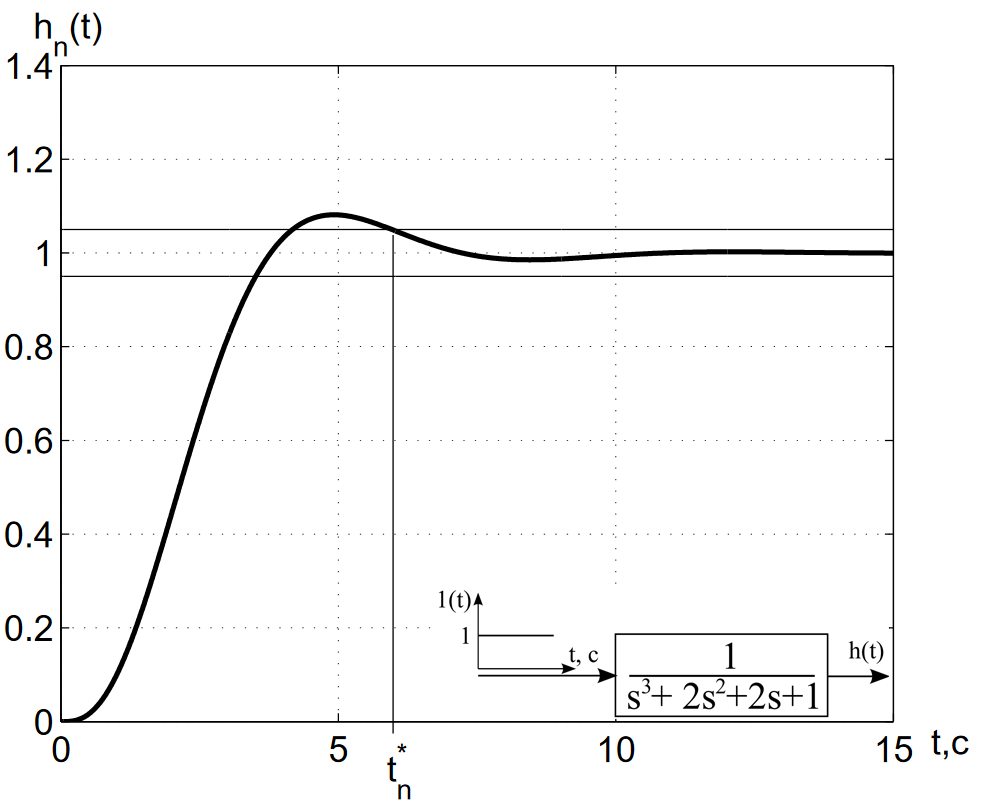
\includegraphics[height = 6cm]{img/buttertime.png}}
	\caption{Определение времени переходного процесса }
	\label{buttertime}
\end{figure}

\begin{figure}[h]
	\noindent\centering{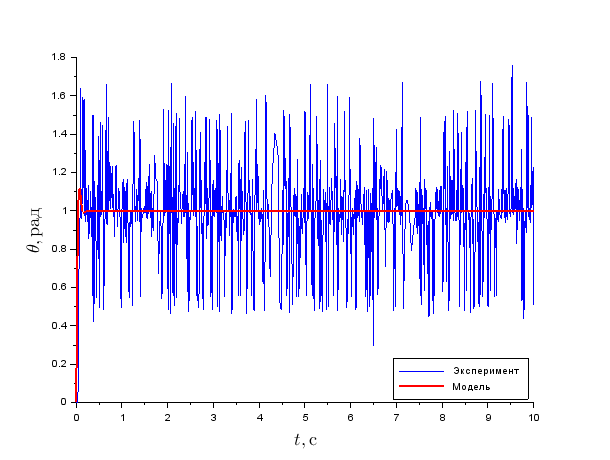
\includegraphics[height = 6cm]{img/B05.png}}
	\caption{График ПИД-регулятора с коэффициентами, полученными из полинома Баттерворта при времени переходного процесса 0.05 сек }
	\label{pidmod2}
\end{figure}

\begin{figure}[h]
	\noindent\centering{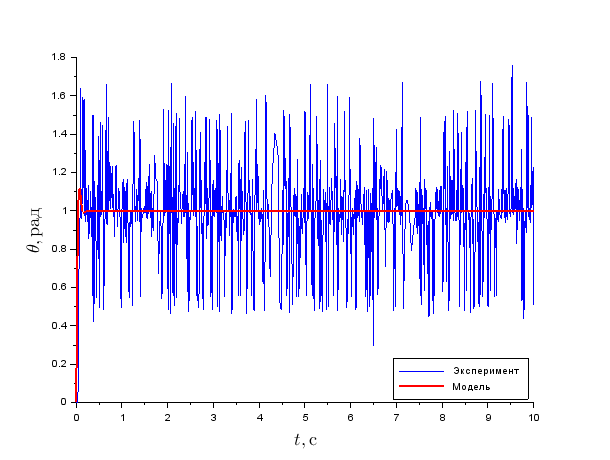
\includegraphics[height = 6cm]{img/B05.png}}
	\caption{График ПИ-регулятора с коэффициентами, полученными из полинома Баттерворта при времени переходного процесса 0.05 сек }
	\label{pimod2}
\end{figure}